\documentclass[a4paper,12pt,twoside]{report} 

\usepackage[utf8]{inputenc}   
\usepackage[T1]{fontenc}           
\usepackage[francais]{babel}  




\usepackage[top=2cm, bottom=2cm, left=2cm, right=2cm]{geometry}

\usepackage{graphicx}
\usepackage{amsmath}
\usepackage{textcomp}
\usepackage[light,math]{kurier}
\setlength{\headheight}{15pt}
\usepackage{lastpage}

\graphicspath{{img/}}

\usepackage{fancyhdr}

\fancyhf{}
\fancyfoot[LE,RO]{\bfseries \thepage} 
\renewcommand{\headrulewidth}{0pt}
\renewcommand{\footrulewidth}{0pt}
\fancyfoot[LO,RE]{Équipe Orga IF}
\fancyfoot[C]{Septembre 2010}

\fancyhead[L]{\bfseries\leftmark}
\fancyhead[R]{\bfseries\rightmark}
\fancyhead[C]{}


\fancypagestyle{plain}{%
\fancyhf{} 
\fancyfoot[RO,LE]{\bfseries \thepage} 
\renewcommand{\headrulewidth}{0pt}
\renewcommand{\footrulewidth}{0pt}}

\fancypagestyle{empty}{%
\fancyhf{} 
\renewcommand{\headrulewidth}{0pt}
\renewcommand{\footrulewidth}{0pt}
}












%pour l'index
\usepackage{makeidx}
\makeindex
                       
%liens hypertexte dans le pdf:
\usepackage{hyperref}
\hypersetup{
    colorlinks,%
    citecolor=black,%
    filecolor=black,%
    linkcolor=black,%
    urlcolor=black
}
\usepackage{bookmark}

%Commandes pour les exigences fonctionnelles
\newcounter{fonction}
\newcommand{\fonction}[1]{
\addtocounter{fonction}{1}
\paragraph{\arabic{fonction} -- {#1}}
}



%%Abbréviations

\def\oh{\emph{Orga Humain}}
\def\24{\emph{24 heures de l'INSA}}



\begin{document}

\pagestyle{fancy} 


\begin{titlepage}



\begin{minipage}{0.3\textwidth}
\centering
\includegraphics[width=3cm]{logobde.jpg}
\\
INSA de Lyon \\
Bureau des Élèves \\

\end{minipage}
\hfill
\begin{minipage}{0.3\textwidth}
\centering
 
~
\\[3cm]

Équipe Orga IF
\end{minipage}


\begin{center} 
\hrulefill \\[0.4cm]
{ \Huge \bfseries PlanningMaker}\\ {  \bfseries Cahier Des Charges Fonctionnel} \\[0.4cm]
 \hrulefill






\vfill {\Large Version 0.2} \\[2cm]
{ Septembre 2010  } \\





\end{center}


\end{titlepage}





\tableofcontents
\addcontentsline{toc}{chapter}{Table des Matières}


\chapter{Introduction}
\section{Présentation du cahier des charges}
Ce cahier des charge présente les attentes du Bureau des Élèves de l'INSA de Lyon, conçernant le développement d'une nouvelle version de PlanningMaker, logiciel
d'aide à la gestion des ressources humaines lors de manifestations.

Ce cahier des charges a été élaboré après avoir consulté les besoins des différentes associations et équipes du BdE susceptibles d'utiliser le logiciel, dont notamment : 
\begin{itemize}
\item Le Comité des Animations
\item Le Comité d'Organisation du Week-End d'Intégration
\item Le Gala
\item Le Raid
\item Les 24 heures de l'INSA de Lyon
\end{itemize}

Ce cahier des charges sera soumis à l'approbation des responsables de ces associations avant le lancement du projet.

\section{Responsables du cahier des charges}
Ce cahier des charges a été rédigé par les personnes suivantes, à contacter pour toute question relative à celui-ci : 
\begin{itemize}
 \item Laurent \textsc{Billon} \texttt{<laurent.billon@insa-lyon.fr>}
\end{itemize}

Il est également possible de contacter directement l'Équipe Orga IF du BdE à l'adresse suivante : \texttt{<bde.equipe.orgaif@insa-lyon.fr>}

\section{Historique des versions}

\begin{description}
\item[v0.1] Intégration des besoins des \24
\end{description}

\chapter{Motivations}
\section{Contexte}
Tout au long de l'année, les associations et les équipes du BdE organisent un grand nombre de manifestations. Lors de leur préparation, la gestion des ressources humaines est un
 élément clé, qui prend souvent un temps considérable. 


\section{Solutions existantes}
Actuellement, un logiciel permettant la gestion des ressources humaines est utilisé sur plusieurs manifestations. Cependant, de nombreuses fonctionnalités sont peu adaptées aux besoins actuels des associations.


\section{Objectif}
Afin de gérer simplement et efficacement la répartition des différentes tâches entre les organisateurs, et permettre la génération de plannings pour ces organisateurs, nous devons
développer une nouvelle version du logiciel PlanningMaker, en prenant compte des nouveaux besoins de utilisateurs.




\chapter{Contraintes}
\section{Temps}
\subsection{Première deadline}
Le logiciel doit être prêt pour pouvoir être utilisé par le \emph{XV\ieme{} Gala de l'INSA de Lyon}, qui aura lieu le 12 février 2011.
\subsection{Échelonnement des exigences}
Compte tenu de la proximité de la deadline, il sera réalisé un échelonnement temporel des livraisons.

Toutes lex exigences fonctionnelles relatives à la gestion des orgas, des tâches, groupes de tâches et commentaires doivent être satisfaites pour le 15 décembre 2010. Une documentation minimale conçernant ces exigences doit être fournie, et une formation devra être dispensée aux futurs utilisateurs.

Toutes les exigences fonctionnelles du logiciel, à l'exception de celles relatives aux véhicules et aux voyages, seront réalisées avant le 15 janvier 2011.

Le logiciel doit être pleinement fonctionnel pour le 15 mars 2011.

\chapter{Définitions et conventions de noms}
\begin{description}
\item[BdE] Bureau des Élèves de l'INSA de Lyon
\item[Manifestation] Événement organisé par une équipe ou une assocuation du BdE.
\item[Orga] Personne effectuant des tâches lors d'une manifestation.
\item[Orga IF] Équipe chargée du système d'information du BdE. Désigne également un membre de cette équipe.

 \end{description}

\chapter{Exigences}
\section{Manifestation}



\fonction{Création}
Le logiciel dispose d'un assistant permettant de se configurer facilement pour une nouvelle manifestation.

Les données sont par la suite entièrement modifiables.



\section{Orgas}



\fonction{Inscription}
Les orgas peuvent insérer leurs propres informations dans le système lors de l'inscription, réalisée à l'aide d'une interface web, accessible en ligne.

\fonction{Modification des Informations}
Les informations fournies par les orgas sont modifiables par eux-mêmes jusqu'à ce qu'elles soient vérouillées.

Le vérrouillage des informations peut être activé manuellement, et il se met en place automatiquement lorsqu'un crénau lui a été assigné.

\fonction{Authentification}
Les orgas peuvent accéder à leurs données et les modifier de manière sécurisée, qu'ils soient ou non étudiants à l'INSA de Lyon.

Il est préférable que les étudiants de l'INSA s'authentifient à l'aide du système CAS.

\fonction{Disponibilités}
Les orgas peuvent déclarer plusieurs plages horaires pendant lesquelles ils peuvent travailler.

\fonction{Amis}
Les orgas peuvent indiquer les personnes avec lesquelles ils souhaitent travailler. Ces souhaits tenterons d'être respectés dans la mesure du possible.

\fonction{Édition de badges}
L'\oh{} peut imprimer des badges pour les orgas.

Les informations pouvant être portées sur les badges sont totalement personnalisables. (Nom de l'orga, catégorie, photo)

Un visuel peut être ajouté et personnalisé.


\fonction{Importation/Exportation}
La liste des orgas, à laquelle on peut ajouter les différentes informations conçernant les orgas (département, etc), peut être exportée vers et importées depuis un format de fichier standard.


\subsection{Lettres d'excuses aux départements}
\fonction{Génération et impression}
Le logiciel permet de générer et d'imprimer des lettres d'excuses adressées aux directeurs des départements.

\fonction{Personnalisation}
Les éléments suivants peuvent être ajoutés et modifiés aux lettres d'excuse : 
\begin{itemize}
\item Plages horaires pendant lesquelles l'orga est excusé (ne mentionner que les heures en semaine)
 \item Nom, adresse, et logotype de l'association
\item Nom et signature du président de l'association.
\item Département et année de l'orga excusé
\item Nom et adresse du destinataire
\item Date
\end{itemize}


\fonction{Administration des orgas}
L' \oh{} peut modifier les informations concernant un orga.


\subsection{Catégories d'orgas}
\fonction{Création}
L'\oh{} peut créer un nombre illimité de catégories d'orgas.

\fonction{Assignation des orgas}
Les orgas peuvent se déclarer comme membre d'une catégorie d'orgas, cette affectation devient active après validation de l'\oh{}. L'Orga ne peut pas voir sa catégorie.

\section{Tâches}

\begin{figure}[h!t]
\centering
\includegraphics[width=\textwidth]{process-tachessvg.png}
\label{fig:ptaches}
\caption{Processus de création et de validation d'un groupe de tâches.}
\end{figure}


\fonction{Création}
Un orga peut créer un nombre illimité de tâches.

\fonction{Validation}
Une tâche peut être validée par le chef de l'équipe à laquelle se rapporte la tâche ou par un \oh{}.

Cette validation doit s'effectuer selon le processus décrit dans la figure \ref{fig:ptaches}

La validation d'une tâche entraîne son vérouillage en écriture.

\fonction{Commentaires}
Un nombre illimité de commentaires peuvent être ajoutés à une tâche par différents orgas humains.


\fonction{Importation/Exportation}
Les tâches (et notamment leurs description) peuvent être exportées vers et importées depuis un format de fichier standard, ainsi que les commentaires qui leur sont associées.


\subsection{Groupe de tâches}
\fonction{Inclusion de tâches}
Une tâche est nécessairement incluse dans un groupe de tâches.
\fonction{Création}
Un orga peut créer un groupe de tâches directement lors de la création d'une nouvelle tâche.

\fonction{Validation}
Un groupe de tâches peut être validée par le chef de l'équipe à laquelle se rapporte la tâche ou par un \oh{}.

Cette validation est similaire à celle d'une tâche.

Il est impossible d'ajouter ou de retirer des tâches à un groupe déjà validé.


\fonction{Commentaires}
Un nombre illimité de commentaires peuvent être ajoutés à un groupe de tâches par différents orgas humains.

\section{Lieux}
\fonction{Création}
Un orga peut créer un lieu directement lors de la création d'une nouvelle tâche.

\fonction{Affichage}
Le logiciel peut générer, et imprimer les états suivants :
\begin{itemize}
 \item Carte globale des lieux
\item Liste des lieux avec mini-carte
\end{itemize}
On tolérera un simple export des lieux vers le logiciel Google Earth\textregistered{}.

\section{Matériel}

\fonction{Création}
Un orga peut créer un matériel directement lors de la création d'une nouvelle tâche.

\fonction{Besoins en Matériel}
L'\oh{} peut générer, visualiser et imprimer la quantité totale de matériel nécessaire, heure par heure.

\fonction{Planning}
L'\oh{} peut générer, visualiser et imprimer le planning d'un matériel.

\section{Créneaux}

\begin{figure}[h!t]
\centering
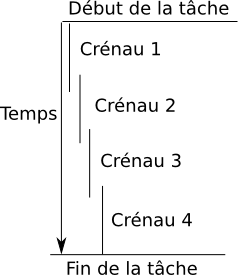
\includegraphics[width=.3\textwidth]{tache-crenaux.png}

\caption{Décomposition d'une tâche en créneaux.}
\label{fig:crenaux}
\end{figure}



\fonction{Création}
Le logiciel peut créer automatiquement des créneaux pour une tâche. Cf figure \ref{fig:crenaux}


\fonction{Planification assistée}
Le logiciel permet de gérer manuellement les assignations de créneaux, en aidant au maximum l'utilisateur dans ses choix.

\fonction{Résultats à produire}
Le logiciel peut générer et afficher les états suivants : 

\begin{itemize}
\item Nombre de créneaux assignés, restant à assigner et orgas disponibles en fonction du temps.
\item Liste des créneaux, triés et groupés indifférament par : 	\begin{itemize}
								  \item Orga
								  \item Équipe
								  \item Horaire
\item Heure
								 \end{itemize}
\item Liste des orgas, triés et groupés indifférament par :  	\begin{itemize}
								  \item Catégorie
								  \item Équipe
								  \item Département
								 \end{itemize}
\item Groupé par tâche, et pour chaque créneau, le lieu du créneau suivant et précédent de l'orga affecté.

\end{itemize}

\fonction{Vérification des erreurs}
Le logiciel affiche une rapport détaillé lorsque une incohérence est détectée dans les créneaux (temps trop court entre deux créneaux, manque d'orgas pour un créneau, tâche sans créneaux, trop peu de temps pour dormir)

La validation des planning suit un ensemble de règles configurables dans le logiciel.

\fonction{Affichage à l'écran}
Le logiciel permet un affichage intéractif des résultats produits, un exemple est présenté dans la figure \ref{fig:interactivite}

\begin{figure}[h!t]
\centering
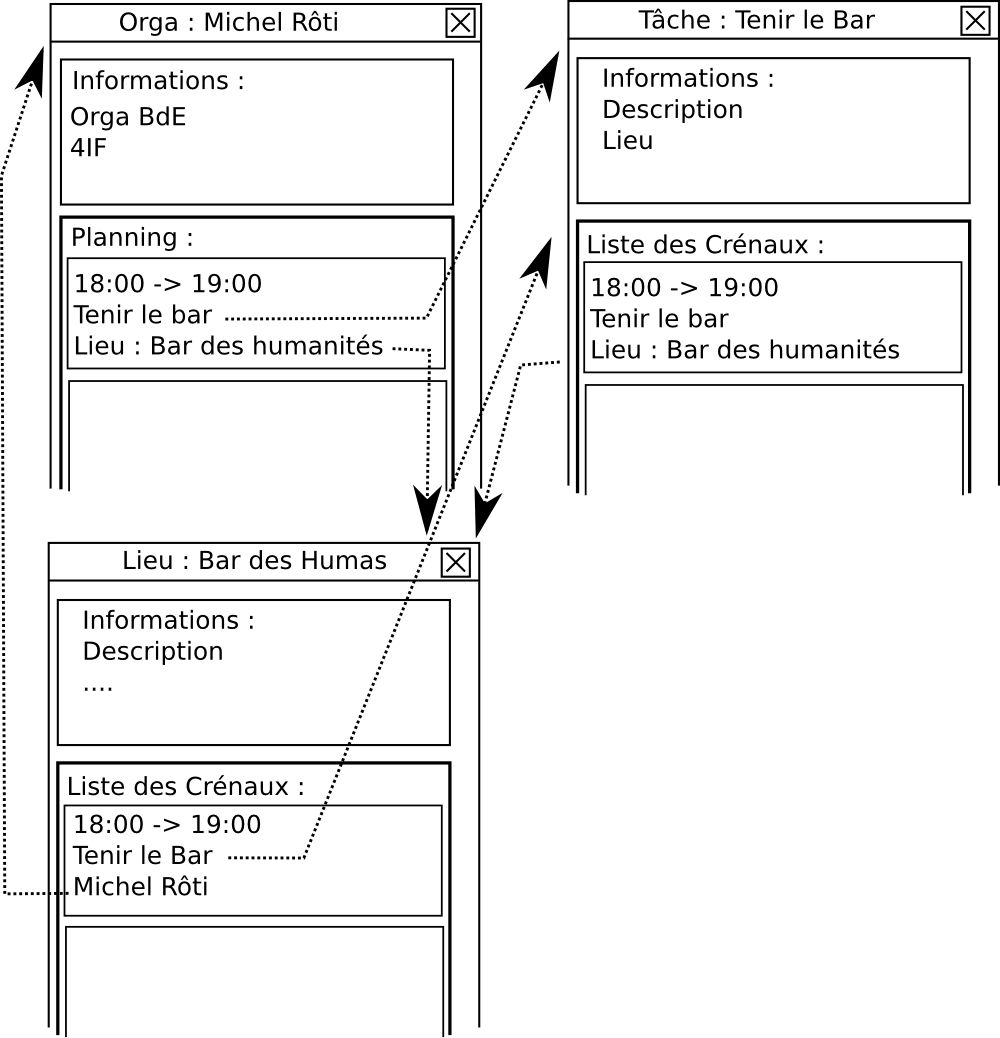
\includegraphics[width=\textwidth]{interactivite.png}

Un clic sur une information ouvre la fenêtre indiquée par la flèche en pointillés..
\caption{Démonstration de l'interactivité}
\label{fig:interactivite}
\end{figure}


\fonction{Affichage de type diagramme de Gantt}
Le logiciel permet d'afficher de manière interactive, sur un affichage de type diagramme de Gantt, la liste des créneaux pour une tâche. Il est possible de faire coincider cet affichage avec l'heure actuelle.
Cf figure \ref{fig:agenda}

\fonction{Export de plannings}
Le logiciel peut exporter le planning d'un utilisateur dans un format ical.

\begin{figure}[h!t]
\centering
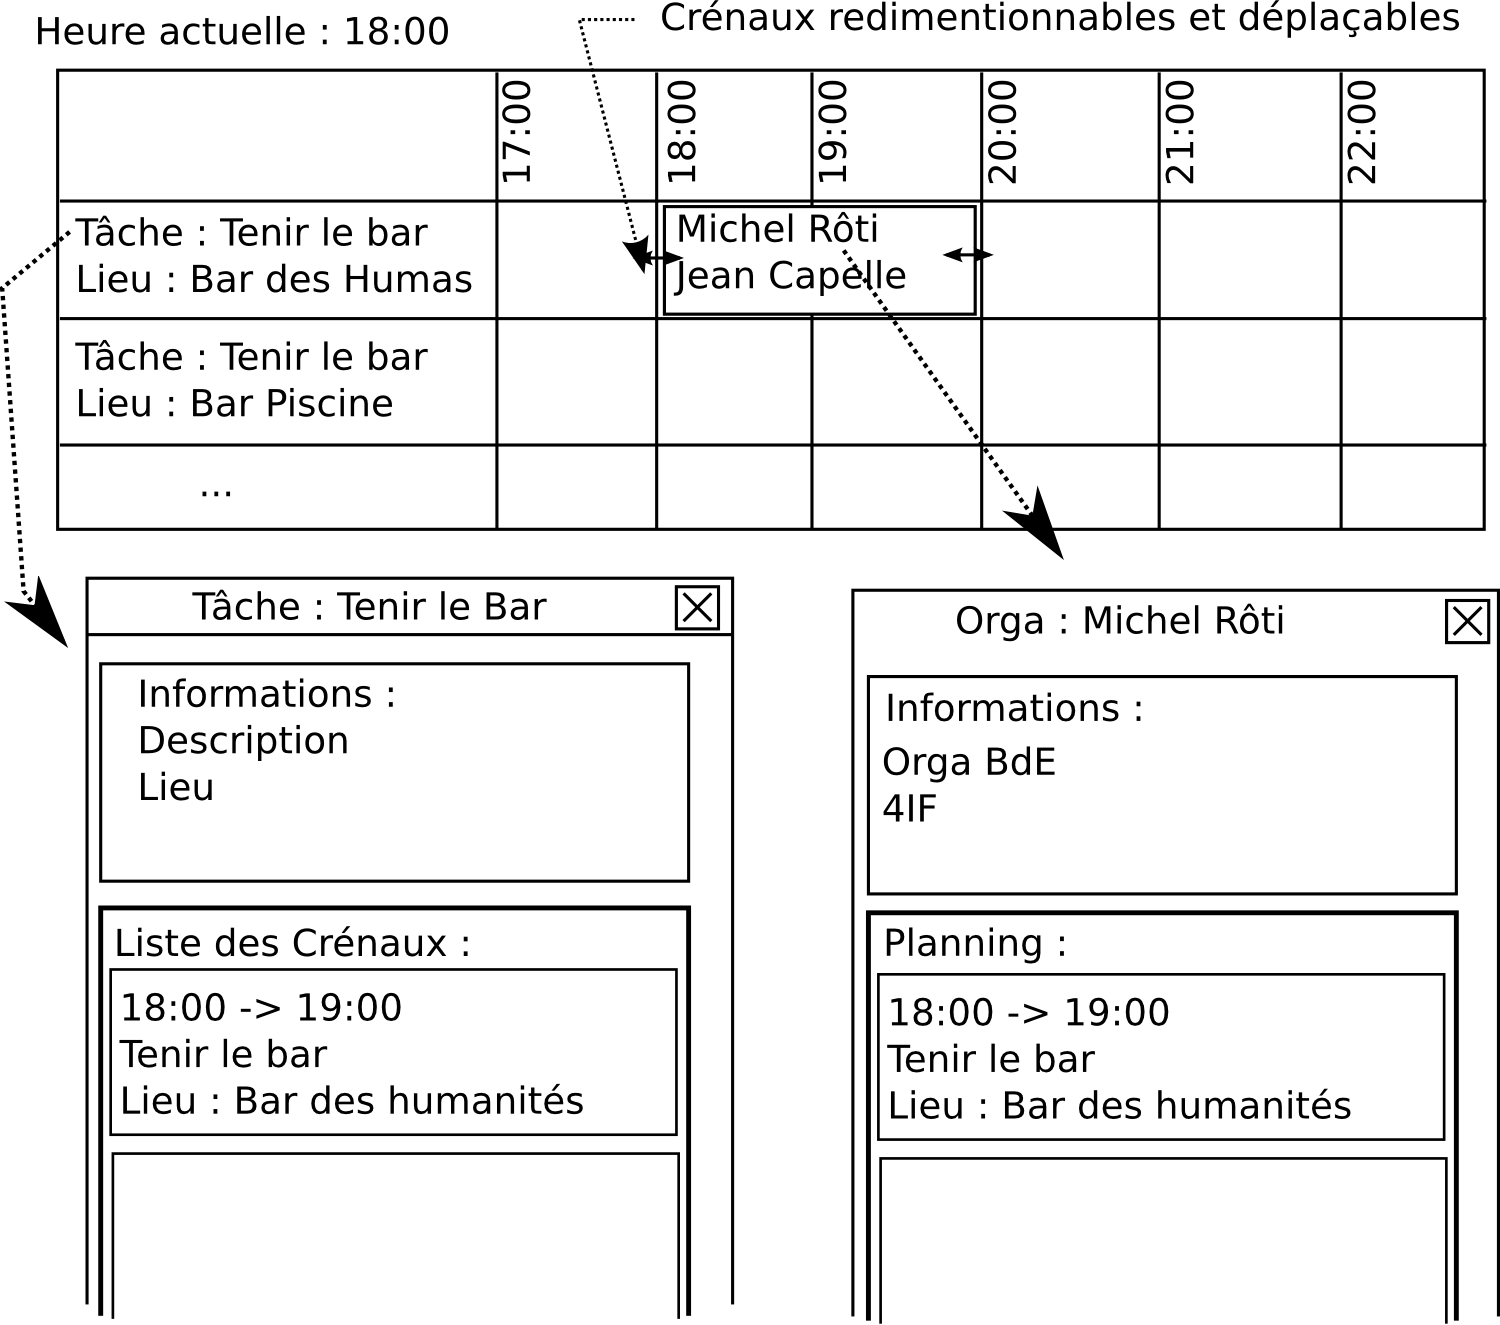
\includegraphics[width=\textwidth]{vue-agenda.png}

\caption{Vue interactive de type diagramme de Gantt}
\label{fig:agenda}
\end{figure}


\fonction{Impression}
Le logiciel peut produire et imprimer tous les résultats produits sous forme adaptée à l'impression, y compris la vue de type diagramme de Gantt.

\fonction{Format des plannings}

Notamment pour les plannings orga, il est possible de personnaliser de manière complète le format des plannings. On peut notamment choisir :
\begin{itemize}
 \item La présentation de chaque créneau (nature et disposition des informations à afficher)
\item Les informations présentées en en-tête, pied de page
\item Les informations présentées à la première et dernière page
\item Les informations présentées au recto du planning (plan de la manifestation par exemple)
\end{itemize}

\section{Véhicule}

\fonction{Création}
Les orgas peuvent créer un nombre illimité de véhicules.


\fonction{Contrôle d'erreurs}
Le logiciel signale à l'utilisateur si un véhicule affecté à une tâche n'est pas présent au lieu de la tâche.





\section{Voyages}

\fonction{Création}
Les orgas peuvent créer un nombre illimité de voyages.

\fonction{Affichage}
Les voyages sont affichés comme des crénaux dans les plannings des orgas.

\fonction{Contrôle de capacité maximale}
Le logiciel signale à l'utilisateur si un véhicule affecté doit transporter plus que sa capacité, en personnes et en matériel.

\subsection{Résultats à produire}
Le logiciel peut générer, afficher de manière interactive et imprimer :
\fonction{Fiche de véhicule ``Véhicule Book''}
Une fiche de véhicule qui indique, pour un véhicule, la liste de ses voyages et toutes les informations qui leurs sont associées, en particulier le matériel à charger.

Pour chaque voyage, un aperçu du trajet peut être donné sous forme de carte.

\fonction{Fiches de transport}
Une fiche de coffre qui indique pour chaque voyage d'un véhicule la liste du matériel et des orgas à transporter.
En en-tête figure les informations spécifiques au voyage et au véhicule.





\pagestyle{fancy} 





%\appendix
%\chapter{Annexes}


%\addcontentsline{toc}{section}{Table des Figures}
%\listoffigures
%\addcontentsline{toc}{section}{Liste des Tableaux}
%\listoftables



\end{document}